\begin{figure}[H]
	\centering
	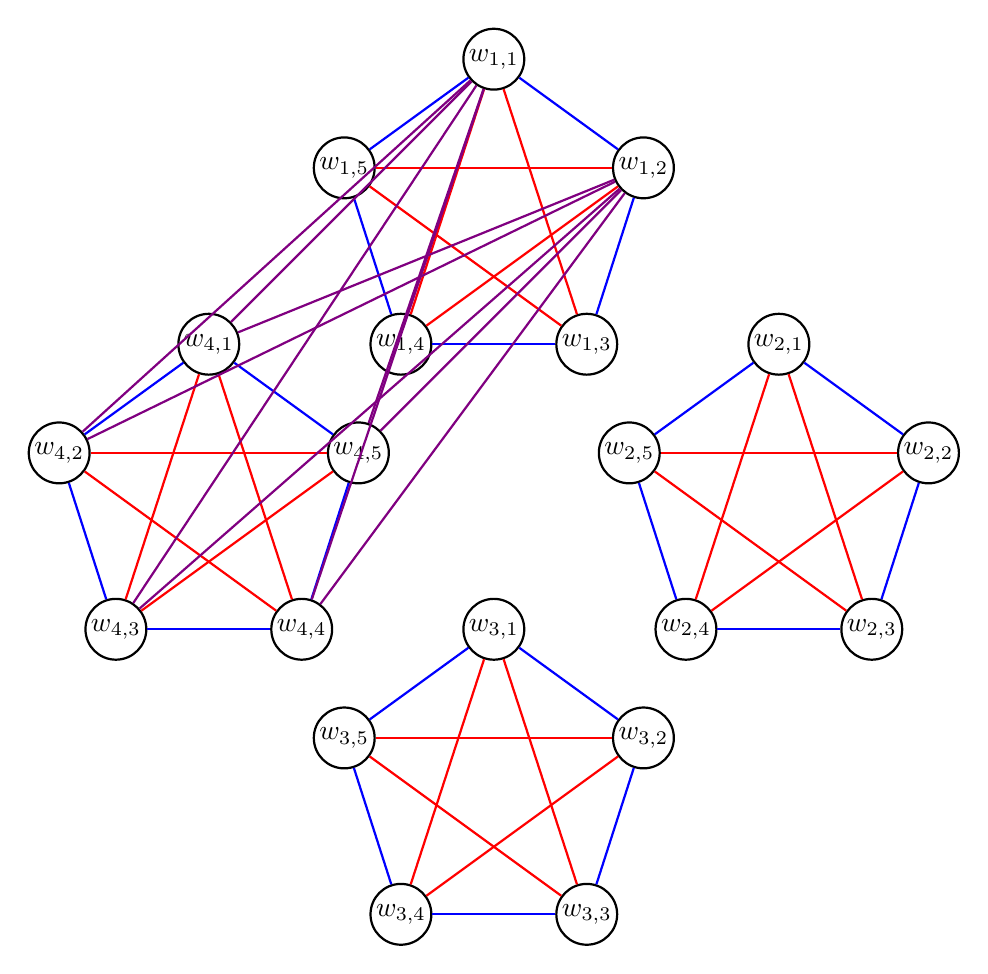
\begin{tikzpicture}
		\tikzset{punkt/.style={circle, thick, draw=black, minimum width=0.2cm,inner sep=1}}
        \node[punkt] at (0.0, 5.62) (a1) {$w_{1, 1}$};
        \node[punkt] at (1.9, 4.24) (b1) {$w_{1, 2}$};
        \node[punkt] at (1.18, 2.0) (c1) {$w_{1, 3}$};
        \node[punkt] at (-1.18, 2.0) (d1) {$w_{1,4}$};
        \node[punkt] at (-1.9, 4.24) (e1) {$w_{1,5}$};

        \node[punkt] at (3.62, 2.0) (a2) {$w_{2, 1}$};
        \node[punkt] at (5.52, 0.62) (b2) {$w_{2, 2}$};
        \node[punkt] at (4.8, -1.62) (c2) {$w_{2, 3}$};
        \node[punkt] at (2.44, -1.62) (d2) {$w_{2, 4}$};
        \node[punkt] at (1.72, 0.62) (e2) {$w_{2, 5}$};

        \node[punkt] at (0.0, -1.62) (a3) {$w_{3, 1}$};
        \node[punkt] at (1.9, -3.0) (b3) {$w_{3, 2}$};
        \node[punkt] at (1.18, -5.24) (c3) {$w_{3, 3}$};
        \node[punkt] at (-1.18, -5.24) (d3) {$w_{3, 4}$};
        \node[punkt] at (-1.9, -3.0) (e3) {$w_{3, 5}$};

        \node[punkt] at (-3.62, 2.0) (a4) {$w_{4, 1}$};
        \node[punkt] at (-5.52, 0.62) (b4) {$w_{4, 2}$};
        \node[punkt] at (-4.8, -1.62) (c4) {$w_{4, 3}$};
        \node[punkt] at (-2.44, -1.62) (d4) {$w_{4, 4}$};
        \node[punkt] at (-1.72, 0.62) (e4) {$w_{4, 5}$};
			\draw [thick, draw=blue] (a1) -- (b1);
			\draw [thick, draw=blue] (b1) -- (c1);
			\draw [thick, draw=blue] (c1) -- (d1);
			\draw [thick, draw=blue] (d1) -- (e1);
			\draw [thick, draw=blue] (e1) -- (a1);

			% Red edges
			\draw [thick, draw=red] (a1) -- (c1);
			\draw [thick, draw=red] (a1) -- (d1);
			\draw [thick, draw=red] (b1) -- (d1);
			\draw [thick, draw=red] (b1) -- (e1);
			\draw [thick, draw=red] (c1) -- (e1);

			\draw [thick, draw=blue] (a2) -- (b2);
			\draw [thick, draw=blue] (b2) -- (c2);
			\draw [thick, draw=blue] (c2) -- (d2);
			\draw [thick, draw=blue] (d2) -- (e2);
			\draw [thick, draw=blue] (e2) -- (a2);

			% Red edges
			\draw [thick, draw=red] (a2) -- (c2);
			\draw [thick, draw=red] (a2) -- (d2);
			\draw [thick, draw=red] (b2) -- (d2);
			\draw [thick, draw=red] (b2) -- (e2);
			\draw [thick, draw=red] (c2) -- (e2);

			\draw [thick, draw=blue] (a3) -- (b3);
			\draw [thick, draw=blue] (b3) -- (c3);
			\draw [thick, draw=blue] (c3) -- (d3);
			\draw [thick, draw=blue] (d3) -- (e3);
			\draw [thick, draw=blue] (e3) -- (a3);

			% Red edges
			\draw [thick, draw=red] (a3) -- (c3);
			\draw [thick, draw=red] (a3) -- (d3);
			\draw [thick, draw=red] (b3) -- (d3);
			\draw [thick, draw=red] (b3) -- (e3);
			\draw [thick, draw=red] (c3) -- (e3);

			\draw [thick, draw=blue] (a4) -- (b4);
			\draw [thick, draw=blue] (b4) -- (c4);
			\draw [thick, draw=blue] (c4) -- (d4);
			\draw [thick, draw=blue] (d4) -- (e4);
			\draw [thick, draw=blue] (e4) -- (a4);

			% Red edges
			\draw [thick, draw=red] (a4) -- (c4);
			\draw [thick, draw=red] (a4) -- (d4);
			\draw [thick, draw=red] (b4) -- (d4);
			\draw [thick, draw=red] (b4) -- (e4);
			\draw [thick, draw=red] (c4) -- (e4);

			\draw[thick, violet] (a1) -- (a4);
			\draw[thick, violet] (a1) -- (b4);
			\draw[thick, violet] (a1) -- (c4);
			\draw[thick, violet] (a1) -- (d4);
			\draw[thick, violet] (a1) -- (e4);

			\draw[thick, violet] (b1) -- (a4);
			\draw[thick, violet] (b1) -- (b4);
			\draw[thick, violet] (b1) -- (c4);
			\draw[thick, violet] (b1) -- (d4);
			\draw[thick, violet] (b1) -- (e4);

			%\draw [thick, violet] (a) -- (d);
			%\draw [thick, draw=violet] (a) -- (b);
			%\draw [thick, draw=violet] (c) -- (d);
			%\draw [thick, draw=green] (b) -- (d);
			%\draw [thick, draw=green] (b) -- (c);
			%\draw [thick, draw=green] (a) -- (c);

	\end{tikzpicture}
	\caption{A graph $G$ with a $2$-edge coloring}
	\label{fig:blow_up_2}
\end{figure}
